
\subsection{\em Fat curve}
Naj bo ${\bf \hat{p}}(t)$ polinom stopnje $k < n$, ki optimalno aproksimira ${\bf f}(t)$ glede na normo $L_2$. Konstruiramo ga s pomočjo nižanja stopnje krivulje ${\bf f}(t)$, podrobnosti o tem kako to naredimo so v \cite{ls_sq}. Sedaj polinomu ${\bf \hat{p}}(t)$ s pomočjo višanja stopnje lahko zvišamo stopnjo do $n$ in zapišemo
$$
{\bf \hat{p}}(t) = {\bf p}(t) = \sum _{i=0}^n {\bf c}_iB_{i,[\alpha,\beta]}^n(t),
$$
kjer so ${\bf c}_i$ nove kontrolne točke. Naj bo 
\begin{equation}\label{def_delta}
\delta = \lVert {\bf f}(t) - {\bf p}(t) \rVert _{BB}^{[\alpha,\beta]}.
\end{equation}
Velja naslednja ocena
$$
\lVert {\bf f}(t) - {\bf p}(t) \rVert = \lVert \sum _{i=0}^n({\bf a}_i-{\bf c}_i)B_{i,[\alpha,\beta]}^n(t) \rVert
\leq \sum _{i=0}^n\lVert{\bf a}_i-{\bf c}_i\rVert B_{i,[\alpha,\beta]}^n(t) \leq \delta.
$$
Sledi, da ${\bf f}(t)$ leži v območju $\mathcal{P}$ med ${\bf p}_1(t) = \hat{{\bf p}}(t) + \delta {\bf n}$ in ${\bf p}_2(t) = \hat{{\bf p}}(t) - \delta {\bf n}$, kjer je ${\bf n}$ normala, ki je pravokotna na ${\bf b}_m - {\bf b}_0$. Območje $\mathcal{P}$ imenujemo {\em fat curve}.
\begin{figure}[!h]
    \centering 
    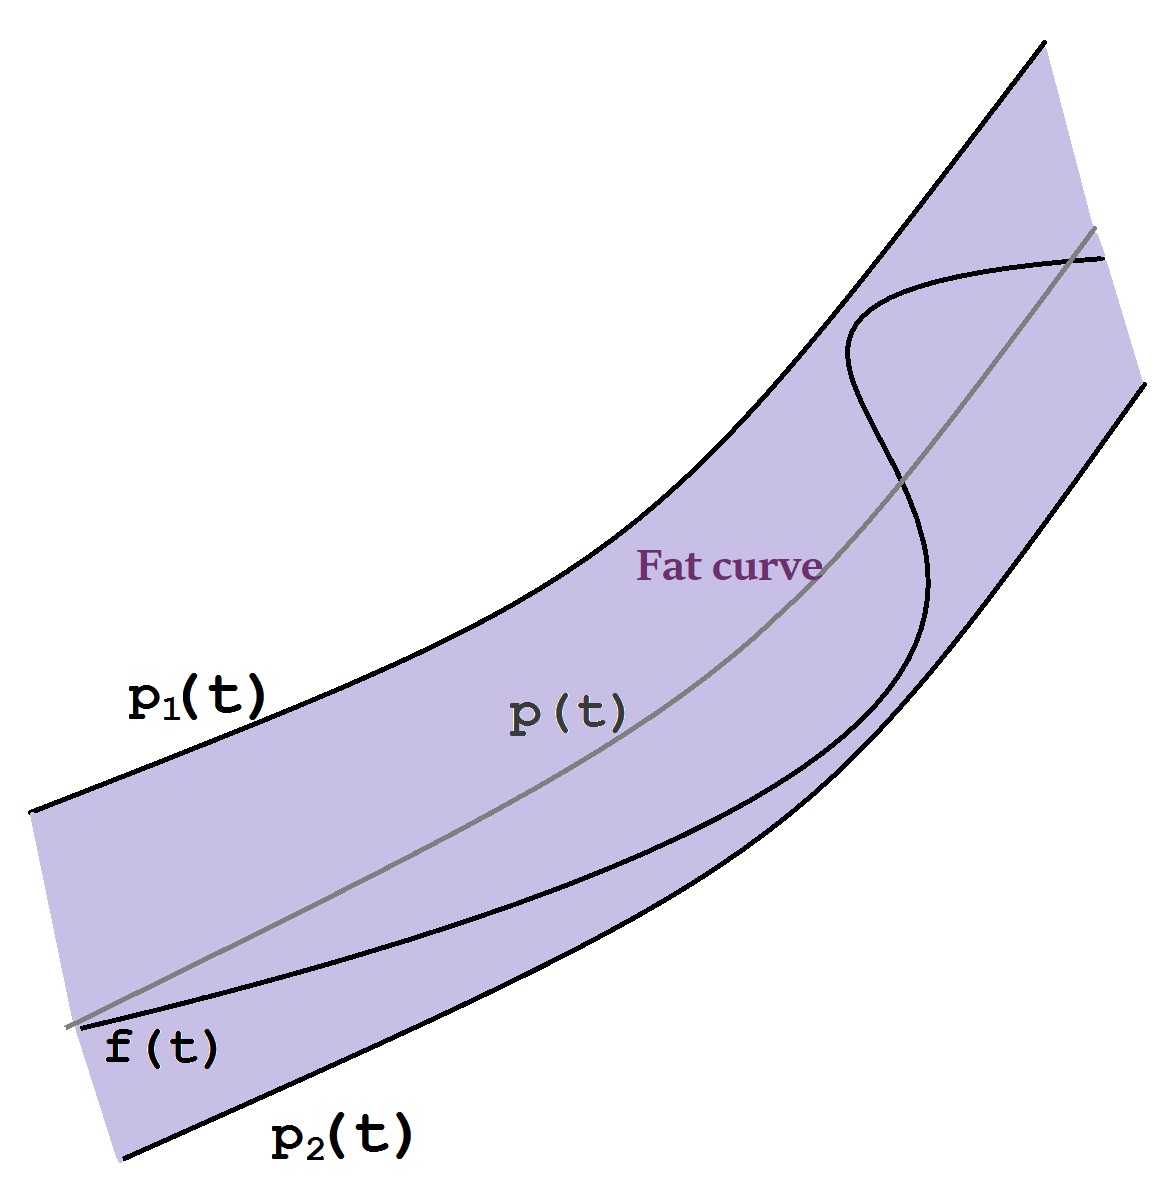
\includegraphics[width=0.44\textwidth]{fat_curve_color}
    \caption{Krivulja {\bf f} in {\em fat curve}.}
  	%\caption{{\em Fat line $\mathcal{L}$}.}
  	\label{slika3}
\end{figure}